\documentclass[a4paper]{report}
\usepackage[utf8]{inputenc}
\usepackage[T1]{fontenc}
\usepackage{RJournal}
\usepackage{amsmath,amssymb,array}
\usepackage{booktabs}

%% load any required packages FOLLOWING this line
\usepackage{bm}
\usepackage[english]{babel}
\usepackage{amsfonts,textcomp}
\usepackage{hhline}
\usepackage{graphics}
\usepackage{geometry}
\usepackage{multirow}
\usepackage{rotating} 
\usepackage{pdflscape}
\usepackage{rotfloat}
\usepackage{subfig}
\usepackage[flushleft]{threeparttable}
\usepackage{ragged2e}
\usepackage{scrextend} % So important!!!


% new mathematical notation
\newcommand{\mA}{\mathcal{A}}
\newcommand{\sign}{\text{sign}}
\newcommand{\0}{\phantom{0}}

\begin{document}

%% do not edit, for illustration only
\sectionhead{Contributed research article}
\volume{14}
\volnumber{1}
\year{2022}
\month{March}
\setcounter{page}{34}

%% replace RJtemplate with your article
\begin{article}
% !TeX root = RJwrapper.tex
\title{A Software Tool For Sparse Estimation Of A General Class Of High-dimensional GLMs}
\author{by Hassan Pazira, Luigi Augugliaro and Ernst C. Wit}

\maketitle

\abstract{
Generalized linear models are the workhorse of many inferential problems. Also in the modern era with high-dimensional settings, such models have been proven to be effective exploratory tools. Most attention has been paid to Gaussian, binomial and Poisson settings, which have efficient computational implementations and where either the dispersion parameter is largely irrelevant or absent. However, general GLMs have dispersion parameters $\phi$ that affect the value of the log-likelihood. This in turn, affects the value of various information criteria such as AIC and BIC, and has a considerable impact on the computation and  selection of the optimal model.%
%
The {R}-package \CRANpkg{dglars} is one of the standard packages to perform high-dimensional analyses for GLMs. Being based on fundamental likelihood considerations, rather than arbitrary penalization, it naturally extends to the general GLM setting. In this paper, we present an improved predictor-corrector (IPC) algorithm for computing the differential geometric least angle regression (dgLARS) solution curve, proposed in \cite{Augug13} and \cite{pazira}. We describe the implementation of a stable estimator of the dispersion parameter proposed in \cite{pazira} for high-dimensional exponential dispersion models. A simulation study is conducted to test the performance of the proposed methods and algorithms. We illustrate the methods using an example. The described improvements have been implemented in a new version of the {R}-package \CRANpkg{dglars}.
}


\section[Introduction]{Introduction}
\label{sec:intro}

High-dimensional inference problems are studies where the number of predictors $p$ for some response variable is larger than the sample size $n$. Modern statistical methods developed to study such high-dimensional data are usually based on combining the objective function with a penalty function (i) to calculate a solution curve embedded in the parameter space and then (ii) to find a point on that curve that represents the best compromise between sparsity and predictive behaviour of the model. The recent statistical literature has a great number of contributions devoted to this problem, such as the $\ell_1$-penalty function \citep{tib96}, the SCAD method \citep{fan01} and the Dantzig selector \citep{cand07}.

\cite{Augug13} proposed a new approach based on the differential geometrical representation of the likelihood, in particular for a generalized linear model (GLM). The method does not require an explicit penalty function and is called differential geometric LARS (dgLARS) because it  generalizes the geometrical ideas on which the least angle regression \citep{efron04} is based.
\cite{pazira} extended the dgLARS method to high-dimensional GLMs with exponential dispersion models and arbitrary link functions. In the same paper, the authors repurposed the classic estimation of the dispersion parameter in a high-dimensional setting and also proposed a new, more efficient estimatator.  \cite{pazira_2} extended the dgLARS method to sparse inference in relative risk regression models.

From a computational point of view, the main problem of the dgLARS method is related to the standard predictor-corrector (PC) algorithm developed by \cite{Augug13} to compute the implicitly defined solution path. The PC algorithm  becomes computationally intractable when working with thousands of variables because in the prediction step, the number of arithmetic operations needed to compute the Euler predictor scales as the cube of the number of variables. 
This leads to a cubic increase in the run time needed for computing the solution curve.


In this paper we briefly explain an improved version of the PC algorithm, proposed in \cite{pazira} and \cite{pazira_3}, simply called the improved PC (IPC) algorithm. The IPC algorithm is able to calculate the solution path in fewer, but more relevant points, greatly reducing the computational burden.
In addition, we use a much more efficient cyclic coordinate descend (CCD) algorithm \citep{Augug12} to calculate a rough dgLARS solution curve for ultra high-dimensional data. In this paper, we focus on the behaviour of the IPC algorithm. The new version of the R-package \CRANpkg{dglars} is implemented with both the CCD and IPC algorithms \citep{Augug14b}. The user can also opt to use the old PC algorithm. The package is available on the Comprehensive {R} Archive Network (CRAN) at \url{http://CRAN.R-project.org/package=dglars}.

The remaining of this paper is organized as follows. Firstly, we briefly review the differential geometry underlying the dgLARS method and briefly explain the dispersion parameter estimation methods. Next, the new functions implemented in the updated version of the {dglars} package are described and shown that they can be used to estimate the dispersion parameter. Then, various simulation studies are performed to evaluate the performance and run times of the proposed estimation algorithms. Finally, we use the functions implemented in the \CRANpkg{dglars} package to illustrate its use in an example data set. 

\section{Methodological Background}
\label{sec:metback}

In this section we describe very briefly the dgLARS method and the dispersion parameter estimation methods. The interested reader is referred to \cite{Augug14a} and \cite{pazira}. In general, the aim of the dgLARS method is to define a continuous model path that attains the highest likelihood with the fewest number of variables.


\subsection[Geometric foundation and formal definition]{Geometric foundation and formal definition}
\label{subsec:dglarsmet}

Let $Y$ be a scalar random variable with probability density function belonging to the exponential family $p(y; \theta,\phi)=\exp\{(y\theta-b(\theta))/a(\phi)+c(y, \phi)\}$, where $\theta \in {\Theta} \subseteq \mathcal{R}$ is called canonical parameter, $\phi \in {\Phi} \subseteq \mathcal{R}^+$ is called dispersion parameter and $a(\cdot)$, $b(\cdot)$ and $c(\cdot,\cdot)$ are specific given functions.
We shall assume that $\Theta$ is an open set. The expected value of $Y$ is related to the canonical parameter by the mean value mapping, namely $\text{E}(Y) = \mu = \tau(\theta) = \partial b(\theta)/\partial \theta$, where $\tau:int(\Theta)\rightarrow\Omega$.
Similarly, the variance of $Y$ is related to its expected value by the identity $\text{Var}(Y) = a(\phi)\text{V}(\mu)$, where $\text{V}(\mu)$ is the variance function. Since $\mu$ is a reparameterization of the model, in the following paper we denote by $p(y; \mu, \phi)$ the probability density function of $Y$. Let $\bm{X}$ be a $p$-dimensional vector of random predictors, a GLM is based on the assumption that the conditional expected value of $Y$ given $\bm{X}$ is specified by the identity
$$
g(\text{E}(Y|\bm{X}))=\beta_0 +\sum_{m=1}^{p} x_m \, \beta_m = \bm x^\top\bm\beta,
$$
where, with a little abuse of notation, $\bm x = (1, x_1, \ldots, x_p)^\top$ and $g(\cdot)$ is called link function. For notation purposes, it is more convenient to denote $g^{-1} (\bm x^\top\bm\beta)$ as $\mu(\bm\beta)$.

When we work with $n$ independent and identically distributed copies of the pair $(Y, \bm{X})$, the marginal distribution of the random vector $\bm{Y}=(Y_1,\ldots,Y_n)^\top$ is an element of the set $\mathcal{S} = \left\{p(\bm{y};\boldsymbol{\mu},\phi) = \right. $ $\left.  \prod_{i=1}^{n} p(y_i;\mu_i,\phi) : \boldsymbol{\mu} \in \Omega^n , \phi \in \mathcal{R}^+ \right\}$, which is a minimal and regular exponential family of order $n$ and can be treated as a differential manifold in which $\boldsymbol{\mu}$ is a coordinate system \citep{Amari85}. At each point of $\mathcal S$ we can attach a tangent space, denoted by $T_{p(\boldsymbol{\mu})}\mathcal{S}$, defined as the as the linear vector space spanned by the $n$ score functions $\partial_i \ell(\boldsymbol{\mu},\phi;\bm{Y}) = \partial\log p(\bm{Y}; \boldsymbol{\mu},\phi)/\partial{\mu}_i$. As suggested in \cite{BurbeaEtAl_JMA_82}, each tangent space can be equipped with an inner product: given two tangent vectors belonging to $T_{\bm{\mu}}\mathcal{S}$, say $v = \sum_{i=1}^n v_i\partial_i \ell(\boldsymbol{\mu},\phi;\bm{Y})$ and $w = \sum_{i=1}^n w_i\partial_i \ell(\boldsymbol{\mu},\phi;\bm{Y})$, their inner product is defined to be:
%
\begin{equation}\label{eqn:inner}
\langle v; w \rangle_{\bm{\mu}} = E_{\bm\mu}(v\cdot w) = \sum_{i=1}^n v_ iw_i E(\{\partial_i \ell(\boldsymbol{\mu},\phi;\bm{Y})\}^2) = \sum_{i=1}^n\frac{v_iw_i}{a(\phi) V(\mu_i)}.
\end{equation}

In order to study the geometrical structure of a GLM, we shall assume that $\boldsymbol{\beta} \rightarrow \{ g^{-1}( \bm{x}_1^\top\boldsymbol{\beta}),\ldots,$ $  g^{-1}( \bm{x}_n^\top\boldsymbol{\beta}) \}^\top = \boldsymbol{\mu}(\boldsymbol{\beta})$ is an embedding, then the set $\mathcal{M}=\{p(\bm{y}; \boldsymbol{\mu}(\boldsymbol{\beta}),\phi) \in \mathcal{S} : \boldsymbol{\beta} \in \mathcal{R}^{p+1}, \, \phi \in \mathcal{R}^+ \}
\label{eq:M}
$ is a $p+1$-dimensional submanifold of $\mathcal{S}$. As previously done, the tangent space of $\mathcal{M}$ at the point $p(\bm{y}; \boldsymbol{\mu}(\boldsymbol{\beta}),\phi)$, denoted by $T_{\boldsymbol{\mu}(\boldsymbol{\beta})}\mathcal{M}$, is the linear vector space spanned by the $p+1$ score functions $\partial_h \ell(\boldsymbol{\beta},\phi;\bm{Y}) = \partial\log p(\bm{Y}; \boldsymbol{\mu}(\boldsymbol{\beta}),\phi)/\partial{\beta}_h$. Since $T_{\boldsymbol{\mu}(\boldsymbol{\beta})}\mathcal{M}$ is a linear subspace of $T_{\boldsymbol{\mu}(\boldsymbol{\beta})}\mathcal{S}$, the inner product (\ref{eqn:inner}) can also be used to define the inner product between two tangent vectors belonging to $T_{\boldsymbol{\mu}(\boldsymbol{\beta})}\mathcal{M}$. For more details see \cite{Augug13} and \cite{pazira_0}.

The dgLARS estimator is based on a differential geometric characterization of the Rao score test statistic, obtained using the inner product between the bases of the tangent space $T_{\boldsymbol{\mu}(\boldsymbol{\beta})}\mathcal{M}$ and the tangent residual vector $\bm{r}(\boldsymbol{\beta}, \phi, \bm{y}; \bm{Y}) = \sum_{i=1}^{n} r_{\boldsymbol{\beta},i} \, \partial_i \ell(\boldsymbol{\beta},\phi; \bm{Y})$, where $r_{\boldsymbol{\beta},i}=y_i-\mu_i(\boldsymbol{\beta})$. Formally, we have the following identity:
%
\begin{align}
\partial_h \ell(\boldsymbol{\beta}, \phi; \bm{Y}) &= \langle \partial_h \ell(\boldsymbol{\beta}, \phi; \bm{Y}) ; \bm{r}(\boldsymbol{\beta}, \phi, \bm{y}; \bm{Y}) \rangle_{\boldsymbol{\mu}(\boldsymbol{\beta})}  \nonumber \\
&= \cos (\rho_h(\boldsymbol{\beta}, \phi)) \cdot ||\bm{r}(\boldsymbol{\beta}, \phi, \bm{y}; \bm{Y}) ||_{\boldsymbol{\mu}(\boldsymbol{\beta})} \cdot \mathcal{I}_{h}^{1/2}(\boldsymbol{\beta}, \phi), 
\label{eq:cos}
\end{align}
where $\mathcal{I}_{h}(\boldsymbol{\beta}, \phi)$ is the Fisher information for $\beta_h$, and $\rho_h(\boldsymbol{\beta}, \phi)$ is a generalization of the Euclidean notion of angle between the $h^{\text{th}}$ column of the design matrix and the residual vector $(r_{\boldsymbol{\beta},i})_{i=\{1, 2,\ldots, n\}}$. Importantly, \eqref{eq:cos}  shows that the gradient of the log-likelihood function does not generalize the equiangularity condition proposed in \cite{efron04} to define the LARS algorithm, since the latter does not consider the variation related to $\mathcal{I}_{h}^{1/2}(\boldsymbol{\beta}, \phi)$, which in the case of a GLM is typically not constant. Using the previous identity, one can see that the signed Rao score test statistic, denoted by $r_{h}(\boldsymbol{\beta}, \phi)$, can be characterized as follows:
%
\begin{align}
r_{h}(\boldsymbol{\beta}, \phi) &= \mathcal{I}^{-1/2}_{h}(\boldsymbol{\beta}, \phi) \cdot \partial_h \ell(\boldsymbol{\beta}, \phi; \bm{Y})   \nonumber \\
&=  \cos(\rho_h(\boldsymbol\beta, \phi)) \cdot \|\bm{r}(\boldsymbol{\beta}, \phi, \bm{y}; \bm{Y}) \|_{\boldsymbol{\mu}(\boldsymbol{\beta})}.
\label{eq:rao}
\end{align}
%
From \eqref{eq:rao} we shall say that two given predictors, say $h$ and $k$, satisfy the generalized equiangularity condition at the point $(\boldsymbol{\beta}, \phi)$ when $|r_{h}(\boldsymbol{\beta}, \phi)|=|r_{k}(\boldsymbol{\beta}, \phi)|$. Inside the dgLARS theory, the generalized equiangularity condition is used to identify the predictors that are included in the active set.

As shown in \cite{pazira}, the Rao score test statistic can be written as
%
$$
r_{h}(\boldsymbol{\beta}, \phi) = (a(\phi))^{-1/2}\frac{\sum_{i=1}^n\partial_h\mu_i(\bm\beta)V^{-1}(\mu_i(\bm\beta))(y_i - \mu_i(\bm\beta))}{\sqrt{\sum_{i=1}^n V^{-1}(\mu_i(\bm\beta))\partial_h\mu_i(\bm\beta))}} = (a(\phi))^{-1/2} r_h(\bm\beta),
$$
then the equiangularity condition and the dgLARS method can be defined using only the function $r_h(\bm\beta)$.

Formally, the dgLARS is a method for constructing a path of solutions, indexed by a positive parameter $\gamma$, where the nonzero estimates of each solution can be defined as follows. For any dataset there exists with probability one a finite decreasing sequence of transitions points, denoted by $\{\gamma^{(j)}\}$. Such that for any $\gamma\in (\gamma^{(j)}; \gamma^{(j-1)})$ the subvector of non-zero estimates, denoted by $\hat{\bm\beta}_\mA(\gamma)$, is defined as the solution to the following non-linear equations
%
\begin{equation}\label{eq:system_dglars}
r_h(\hat{\bm\beta}_\mA(\gamma)) -  s_h \gamma = 0, \quad\forall\,h\in\mA,
\end{equation}
%
where $\mA = \{h\,:\, \hat\beta_{h}(\gamma)\neq0\}$ is called active set and $s_h = \sign(r_h(\hat{\bm\beta}_\mA(\gamma)))$. Furthermore, for any $k\notin\mA$ we have that $|r_k(\hat{\bm\beta}(\gamma))| < \gamma$. 

At each transition point we have a change in the active set. We shall say that $\gamma^{(j)}$ is an inclusion transition point if there exists $k\notin\mA$ such that the equiangularity condition is satisfied, which can also be written as
%
\begin{equation}\label{eq:gin}
|r_k(\hat{\bm\beta}_\mA(\gamma^{(j)}))| = \gamma^{(j)}.
\end{equation}
%
In this case the active set is updated adding the index $k$, i.e. the predictor $X_k$ is included in the current model. As explained in \cite{Augug13}, a generalization of the lasso estimator can be obtained letting $s_h = \sign(\hat\beta_h(\gamma))$, in this way a predictor will be removed from the current model when the sign of the the associated estimate is not in agreement with the sign of the Rao score test statistic. Formally, we shall say that $\gamma^{(j)}$ is an exclusion transition point if there exists $h\in\mA$ such that the following condition is satisfied:
%
\begin{equation}\label{eq:gout}
\sign(r_h(\hat{\bm\beta}_\mA(\gamma^{(j)}))) \ne s_h.
\end{equation}
%
In this case the active set is updated removing the index $h$ and $X_h$ is removed from the current model. In Table \ref{tab:ipc} the pseudo-code of the improved PC  algorithm is reported. 
In order to distinguish between the two generalizations, in this paper the first one is called dgLARS and dgLASSO denotes the generalization of the lasso estimator.


\subsection[Computational aspects: the improved PC algorithm]{Computational aspects: the improved PC algorithm}
\label{subsec:estdglars}





\begin{table*}[t!]
	\caption{Pseudo-code of the IPC algorithm to compute the dgLARS and dgLASSO solution curves.} 
	\centering
	\renewcommand\arraystretch{1.4}
	%\renewcommand\tabcolsep{2pt}
	\begin{tabular}{ccp{12cm}}
		\hline
		Step && Algorithm  \\
		\cline{1-1}  \cline{3-3}
		
		1 &&  First compute  $\hat{{\beta}}_{0}$ \\ %$\hat{\beta}_{a_0}$ and then compute $\hat{\phi}_{_0}$ at $(\hat{\beta}_{a_0},0,\ldots, 0)^\top$\\ %\hat{\boldsymbol{\beta}}_0=
		
		2 && Set $\mathcal{A} \leftarrow \arg\max_{k \notin \mathcal{A}} \{ |r_{k}(\hat{{\beta}}_{{0}})| \} \ \text{and} \ \gamma \leftarrow |r_{h \in \mathcal{A}}(\hat{{\beta}}_{{0}})| $  \\
		
		3 && Repeat   \\
		
		4 && \hspace{0.1in}  Use \eqref{eq:delta_in} to compute $\triangle \gamma^{in}$ and set $\triangle \gamma \leftarrow \triangle \gamma^{in}$ \\
		
		5 && \hspace{0.1in}  If method = ``dgLASSO'' then \\
		
		6 && \hspace{0.3in} use \eqref{eq:delta_out} and then \eqref{eq:delta_in_out} to compute $\triangle \gamma^{out}$ and $\triangle \bar\gamma$, respectively, and  \\
		
		7 && \hspace{0.3in} set $\triangle \gamma \leftarrow \triangle \bar\gamma$ \\
		
		8 && \hspace{0.1in}  Set $\gamma \leftarrow \gamma-\triangle \gamma$ \\
		
		9 && \hspace{0.1in} Use \eqref{eq:euler_pred} to compute $\tilde{\boldsymbol{\beta}}_{\mathcal{A}}(\gamma)$ \ \ \  (\textit{predictor step}) \\
		
		10 && \hspace{0.1in} Use $\tilde{\boldsymbol{\beta}}_{\mathcal{A}}(\gamma)$ as starting point to solve system \eqref{eq:system_dglars} \ (\textit{corrector step}) \\
		
		%7 && \hspace{0.1in} Compute $\hat{\phi}$ at $\hat{\boldsymbol{\beta}}_{\mathcal{A}}(\gamma)$ \\
		
		11 && \hspace{0.1in} For all $k \notin \mathcal{A}$ compute $r_{k}(\hat{\boldsymbol{\beta}}_{\mathcal{A}}(\gamma))$  \\
		
		12 && \hspace{0.1in} If $\exists k \notin \mathcal{A}$ such that $\left|r_{k}(\hat{\boldsymbol{\beta}}_{\mathcal{A}}(\gamma) ) \right| > \gamma$ then \\
		
		13 && \hspace{0.3in} use \eqref{eq:mystepsize5} to compute $\gamma_{k}^{rf (l)}$ and set $\gamma_{k}^{rf} \leftarrow \underset{l}{\max} \{ \gamma_{k}^{rf (l)} \}$  \\
		
		14 && \hspace{0.3in} first set $\triangle \gamma \leftarrow \triangle \bar\gamma - (\gamma_{k}^{rf}-\gamma)$ and then $\gamma \leftarrow \gamma_{k}^{rf}$, and go to step $\textrm{9}$   \\
		
		15 && \hspace{0.1in} If $ \exists k \notin \mathcal{A}  \ \text{such that} \ \left|r_{k}(\hat{\boldsymbol{\beta}}_{\mathcal{A}}(\gamma))\right| = \left|r_{h}(\hat{\boldsymbol{\beta}}_{\mathcal{A}}(\gamma))\right|$ for all $ h \in \mathcal{A}(\gamma) $, then \\
		
		16 && \hspace{0.3in} update $\mathcal{A}(\gamma)$ \\
		
		17 && Until convergence \\
		\hline
	\end{tabular}
	\label{tab:ipc}
	\medskip
\end{table*}


Computationally, the problem of how to estimate the dgLARS solution curve can be decomposed into two sub-problems. The first defines an efficient computational method to compute the transition points, i.e., the values of the tuning parameter corresponding to a change in the active set. In other words, at each transition points, say $\gamma^{(j)}$, only one of condition (\ref{eq:gin}) or (\ref{eq:gout}) is satisfied. Note that condition (\ref{eq:gout}) is only used when the generalization of the lasso estimator is considered. The second problem is to define an efficient computational method to compute the path of solutions when $\gamma\in (\gamma^{(j)}; \gamma^{(j-1)})$. This sub-problem requires the solution to the following system of non-linear equations:
$$
r_h(\hat{\bm\beta}_\mA(\gamma)) -  s_h \gamma= 0, \quad\forall\,h\in\mA,
$$
with $\gamma\in (\gamma^{(j)}; \gamma^{(j-1)})$ and where $s_h = \sign(r_h(\hat{\bm\beta}_\mA(\gamma)))$ if we want to compute the dgLARS solution curve or $s_h = \sign(\hat\beta_h(\gamma))$ if the dgLASSO solution curve is required.

\cite{Augug13} proposed a predictor-corrector (PC) algorithm to solve the two sub-problems. Although this algorithm can compute the solution curve for moderately large problems, identifying the transition points is extremely inefficient and can led to a significant increase in computational time. This problem is highlighted in \cite{pazira} and \cite{pazira_3}, where an improvement to the original PC algorithm is also proposed. In order to make this paper self-contained, we briefly review this algorithm.

Let $\boldsymbol{\tilde{\varphi}}_{\mA}(\gamma)=\boldsymbol{{\varphi}}_{\mA}(\gamma)- \bm{s}_{\mA}\gamma$, where $ \boldsymbol{{\varphi}}_{\mA}(\gamma) = (r_h(\hat{\bm{\beta}_\mA}(\gamma)))_{h\in\mA}^\top $ and $ \bm{s}_{\mathcal{A}}=(s_h)_{h\in\mA}^\top$. Suppose we have computed the solution of the system (\ref{eq:system_dglars}) at $\gamma$, denoted by $\bm{\hat\beta}_\mA(\gamma)$, and we want to compute the next solution at $\gamma - \Delta\gamma\in(\gamma^{(j)};\gamma^{(j - 1)})$. In the predictor step, the new solution is approximated by the following expression:
%
\begin{equation}\label{eq:euler_pred}
\bm{\hat{\beta}}_{\mA}(\gamma - \Delta \gamma) \approx \bm{\tilde{\beta}}_{\mA}(\gamma - \Delta \gamma)=\bm{\hat{\beta}}_{\mA}(\gamma)- \Delta \gamma \ \Im_\mA^{-1} (\gamma) \ \bm{s}_\mA,
\end{equation}
%
where $\Im_\mA(\gamma)$ is the Jacobian matrix of the vector function $\bm{\varphi}_\mA(\gamma)$ evaluated at  $\bm{\hat{\beta}}_\mA(\gamma)$. In the corrector step, the approximation (\ref{eq:euler_pred}) is used as the starting point of the algorithm solving the system of non-linear equations:
$$
r_h(\hat{\bm\beta}_\mA(\gamma-\Delta\gamma)) - s_h (\gamma - \Delta\gamma)  = 0, \quad\forall\,h\in\mA.
$$
In order to reduce the computational burden needed to compute the entire path of solutions, $\Delta\gamma$ is chosen in such a way that at $\hat{\bm\beta}_\mA(\gamma-\Delta\gamma)$ there is a change in the current active set. After straightforward algebra, $\gamma^{(j)}$ can be approximated by $\gamma^{(j - 1)} -\Delta\gamma^{\text{in}}$ where the step size $\Delta\gamma^{\text{in}}$ is equal to:
\begin{equation}\label{eq:delta_in}
\Delta\gamma^{\text{in}} = \min_{k\notin\mA} \left\{\frac{\gamma - r_k(\hat{\bm\beta}_\mA(\gamma))}{1 - \text{d}r_k(\hat{\bm\beta}_\mA(\gamma))/\text d\gamma}; \frac{\gamma + r_k(\hat{\bm\beta}_\mA(\gamma))}{1 + \text{d}r_k(\hat{\bm\beta}_\mA(\gamma))/\text d\gamma}\right\}_+.
\end{equation}
When we want to compute the dgLASSO solution curve, exclusion condition (\ref{eq:gout}) must be added in the computation of the step size. Since the sign of a Rao score test associated with a predictor included in the current model never changes, condition \eqref{eq:gout} is equivalent to the following condition: $\gamma^{(j)}$ is an exclusion transition point if there exists a $h\in\mA$ such that
$
\hat\beta_h(\gamma^{(j)}) = 0.
$
Combining approximation~(\ref{eq:euler_pred}) with the previous condition, it is easy to see that the step size corresponding to the first exclusion can be approximated by the quantity
\begin{equation}\label{eq:delta_out}
\Delta\gamma^{\text{out}} = \min_{h\in\mA}\{\hat\beta_h(\gamma) / d_h(\gamma)\},
\end{equation}
where $\bm d_\mA(\gamma) =  \Im_\mA^{-1} (\gamma) \ \bm{s}_\mA$. Then the step size for the dgLASSO solution curve can be approximated by the quantity
\begin{equation}\label{eq:delta_in_out}
\Delta\bar{\gamma} = \min\{\Delta\gamma^{\text{in}}; \Delta\gamma^{\text{out}}\}.
\end{equation}

Since the step size $\Delta\gamma^{\text{in}}$ and $\Delta\gamma^{\text{out}}$ are obtained using the approximation~(\ref{eq:euler_pred}), we also include an exclusion step for removing incorrectly included variables in the model. Determining how to implement this exclusion step is the main difference between the PC and IPC algorithms. When an incorrect variable is included in the model after the corrector step, there exists a non-active variable such that the absolute value of the corresponding Rao score test statistic is greater than $\gamma$. In this case, the original PC algorithm reduces the step size using a contractor factor $\mbox{cf}$, whereas the IPC algorithm applies the Regula-Falsi ($\mbox{rf}$) method. This method uses information about the function $\tilde\varphi_k(\gamma) = r_k(\hat\beta_\mA(\gamma)) - \gamma s_k$,  draws a secant from $\tilde\varphi_k(\gamma_{new})$ to $\tilde\varphi_k(\gamma_{old})$, and estimates the root as where it crosses the $\gamma$-axis. 

From (\ref{eq:system_dglars}), we know that  $r_{h} (\bm{\hat\beta}_\mA(\gamma))-s_h \gamma = 0$ for all $h\in\mA$. Indeed, after the corrector step, when there are non-active variables such that the absolute value of the corresponding Rao score test statistic is greater than $ \gamma$, we want to find a point, $\gamma^{rf}$ that is close to the true point transition point, reducing the number of the points of the solution curve.
It is easy to verify that the root $\gamma^{rf}_k$ is given by
%
\begin{align}
\gamma^{rf}_k = \frac{r_{k} (\bm{\hat\beta}_\mA(\gamma_{old})) \ \gamma_{new} -  r_{k} (\bm{\hat\beta}_\mA(\gamma_{new})) \ \gamma_{old} }{ r_k (\bm{\hat\beta}_\mA(\gamma_{old}))- r_k (\bm{\hat\beta}_\mA(\gamma_{new}))+  (\gamma_{new}-\gamma_{old}) \ s_k}, 
\hspace{0.2in} \forall k \notin \mA
\label{eq:mystepsize5}
\end{align}
%
where  $ s_k= \text{sign}\{r_k(\bm{\hat\beta}_\mA(\gamma_{new}))\}$. Then the optimal step size is defined as
%
$$
\gamma^{rf} = \{\gamma^{rf}_k\;:\; |r_k (\bm{\hat\beta}_\mA(\gamma))| > \gamma\}.
$$
In total, the main difference between the PC and IPC algorithms is the different techniques used for adjusting the step size to find the transition points. In At the end of next section we examine the performance of the IPC algorithm and compare it to the original PC algorithm by using the functions in the \CRANpkg{dglars} package.




\subsection[Estimation of the dispersion parameter]{Estimation of the dispersion parameter}
\label{subsec:estdisp}

Since the dispersion parameter $\phi$ affects the value of the log-likelihood function, it also impacts the value of various information criteria such as AIC and BIC. Therefore, model selection considerations need to take into account the estimation of the dispersion parameter. 
There are three commonly-used estimators of the dispersion parameter for ordinary GLMs: deviance, maximum likelihood and Pearson estimators \citep{mcc89}. For high-dimensional GLMs, \cite{pazira} proposed two alternative estimators. The first is a generalized version of the Pearson estimator, $\hat{\phi}_{_{P}}(\gamma)$, 
\begin{align}
\hat{\phi}_{_{P}}(\gamma) = \frac{1}{n-|\mA|}\sum^n_{i=1}\frac{(y_i-g^{-1}(\bm{x}_i^\top \boldsymbol{\hat{\beta}}_{\mathcal{A}}(\gamma) ))^2}{V(g^{-1}(\bm{x}_i^\top \boldsymbol{\hat{\beta}}_{\mathcal{A}}(\gamma)))}.
\label{eq:pearson5}
\end{align}
This estimator is fast, but can be improved by the second proposal of an iterative procedure, called General Refitted Cross-Validation (GRCV), to attenuate the influence of irrelevant variables with high spurious correlations. 

The idea of the GRCV method is to split the data ($\bm{y}_{n}, \bm{X}_{n \times p}$) randomly into two equal halves ($\bm{y}_{n_1}^{(1)}, \bm{X}^{(1)}_{n_1 \times p}$) and ($\bm{y}_{n_2}^{(2)}, \bm{X}^{(2)}_{n_2 \times p}$). Where we assume that the sample size $n$ is even and $n_1=n_2=n/2$.
In the first stage, the dgLARS method is applied to these two data sets separately to estimate two solution paths $\boldsymbol{\hat{\beta}}_{{\mathcal{A}}_j}(\gamma)$ based on ($\bm{y}^{(j)}, \bm{X}^{(j)}$) where $j=\{1, 2 \}$ and $|{\mathcal{A}}_j| \leq \min(\frac{n}{2}-1,p)$.

In the second stage, we perform model selection on each training set to determine two small subsets of selected variables $\hat{\mathcal{A}}_1 \subseteq {\mathcal{A}}_1$ and $\hat{\mathcal{A}}_2 \subseteq {\mathcal{A}}_2$.
To do that, we estimate $\phi$ by the generalized Pearson estimator \eqref{eq:pearson5} on these two data sets separately to obtain valid log-likelihood functions $ \ell (\boldsymbol{\hat{\beta}}_{\mathcal{A}_1}(\gamma),\hat{\phi}_{_{P}}^{(1)}(\gamma);\bm{y}^{(1)}) $ and $ \ell (\boldsymbol{\hat{\beta}}_{\mathcal{A}_2}(\gamma),\hat{\phi}_{_{P}}^{(2)}(\gamma);\bm{y}^{(2)}) $.

In the third stage, the coefficient $\boldsymbol{\beta}$ for each subset of the data are re-estimated using the variables selected on the other subset, i.e., ($\bm{y}^{(2)}, \bm{X}^{(2)}_{\hat{\mathcal{A}}_1}$) and ($\bm{y}^{(1)}, \bm{X}^{(1)}_{\hat{\mathcal{A}}_2}$). Since the MLE may not always exist, in this stage we propose to use the dgLARS method to estimate the coefficients based on the selected variables $\hat{\boldsymbol{\beta}}_{\hat{\mathcal{A}}_1}(\gamma_{0}) $ and $\hat{\boldsymbol{\beta}}_{\hat{\mathcal{A}}_2}(\gamma_{0}) $ where $ \gamma_{0}$ is close to zero. If the MLE does exist, then the dgLARS estimate $\hat{\boldsymbol{\beta}}_{{\mathcal{A}}}(0) $ is equal to the MLE.

\begin{figure}[t!]
	\hbox{\hspace{2em}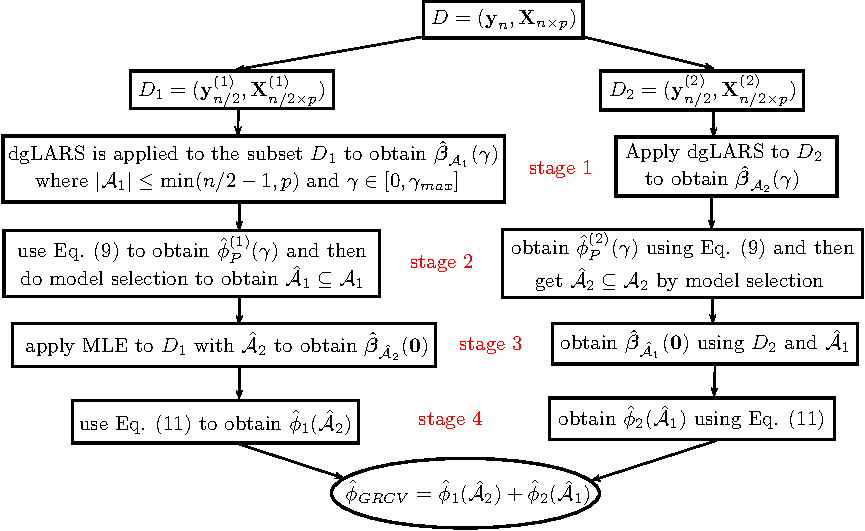
\includegraphics[width=0.9\textwidth]{grcv.pdf}}
	\caption{A general diagram for obtaining the GRCV estimate, a four-stage refitted procedure.}
	\label{fig:grcv}
\end{figure}


Finally, in the fourth stage, we estimate the dispersion parameter $\phi$ by the following estimator on the two data sets ($\bm{y}^{(2)}, \bm{X}^{(2)}_{\hat{\mathcal{A}}_1}$) and ($\bm{y}^{(1)}, \bm{X}^{(1)}_{\hat{\mathcal{A}}_2}$);
\begin{align}
\hat{\phi}_{_{GRCV}}(\hat{\mathcal{A}}_1,\hat{\mathcal{A}}_2) = {\hat{\phi}_{1}(\hat{\mathcal{A}}_2)+\hat{\phi}_{2}(\hat{\mathcal{A}}_1)},
\label{eq:fan3}
\end{align}
where
\begin{align}
\hat{\phi}_{\zeta}(\hat{\mathcal{A}}_j) = \frac{1}{{n}-2 | \hat{\mathcal{A}}_j|} \sum^{\frac{n}{2}}_{i=1}\frac{\left( y^{(\zeta)}_i-g^{-1}\left( (\bm{x}_{i,\hat{\mathcal{A}}_j}^{(\zeta)\top} \ \hat{\boldsymbol{\beta}}_{\hat{\mathcal{A}}_j}(0) \right) \right) ^2}{V\left( g^{-1}\left( \bm{x}_{i,\hat{\mathcal{A}}_j}^{(\zeta) \top} \  \hat{\boldsymbol{\beta}}_{\hat{\mathcal{A}}_j}(0)\right) \right) }, \ \ \ \zeta \neq j
\label{eq:fan}
\end{align}
$\bm{x}_{i,\hat{\mathcal{A}}_j}^{(\zeta)}$ is the $i^{\text{th}}$ row of the $\zeta^{\text{th}}$ subset of the data $ \bm{X}^{(\zeta)}_{\hat{\mathcal{A}}_j}$, $|\hat{\mathcal{A}}_j|$ denotes the cardinality of the set $\hat{\mathcal{A}}_j$, $\hat{\boldsymbol{\beta}}_{\hat{\mathcal{A}}_j}(\gamma) $ is the dgLARS estimator at $\gamma \in [ 0,\gamma_{max}]$, $\hat{\boldsymbol{\beta}}_{\hat{\mathcal{A}}_j}(0)$ is the ML estimate of ${\boldsymbol{\beta}}_{\hat{\mathcal{A}}_j}$, $j=\{1, 2 \}$ and $\zeta=\{1, 2 \}$. 


Figure~\ref{fig:grcv} describes the four step procedure for calculating the GRCV estimate of the dispersion parameter. Since in the second stage of the GRCV procedure the dispersion parameter has to be estimated, an iterative procedure can be defined to reduce its dependence on the generalized Pearson estimator: The algorithm iterates the four steps, such that for the $(\kappa+1)^{\text{th}}$ iteration the $\kappa^{\text{th}}$ GRCV estimate ($\hat{\phi}^{ ^{(\kappa)}}_{_{GRCV}}$) is used to compute the new $(\kappa+1)^{\text{th}}$ GRCV estimate ($\hat{\phi}^{ ^{(\kappa+1)}}_{_{GRCV}}$), and so on. Furthermore due to the random cross-validation splits, the estimate contains random variation, and the algorithm will not numerically converge. Therefore, the median of the final  iterates can be used as the final GRCV estimate ($\hat{\phi}^*_{_{GRCV}}$).

\cite{pazira} showed that the GRCV estimator $\hat{\phi}^*_{_{GRCV}}$ is more stable and accurate, which leads to improved overall model selection behaviour.  

\bigskip

\section[The dglars package]{The \CRANpkg{{dglars}} package: new features}
\label{sec:dglarspkg}

The \CRANpkg{dglars} package \citep{Augug14b} is a collection of computational tools related to the inference procedure of the dgLARS method in the {R} programming environment. % \citep{r12}

\subsection[Description of the dglars() function]{Description of the new \code{dglars()} function}

Different from the previous version, the new \CRANpkg{dglars} package (version $2.1.6$) supports the \code{gaussian}, \code{binomial}, \code{poisson}, \code{Gamma} and \code{inverse.gaussian} families with the most commonly used link functions. The main function of this package, \code{dglars()}, is a wrapper function implemented to handle the formula interface usually used in {R} to create the $n \times p$ model matrix $X$ and the $n$-dimensional response vector $y$;

\begin{example}
dglars(formula, family = gaussian, g, unpenalized, b_wght, data, subset,
       contrast = NULL, control = list())
\end{example}

This function is used to compute the dgLARS/dgLASSO solution curve. As in the standard \code{glm} function, the user can specify the family and link functions using the argument \code{family}; see the next section regarding an example of Gamma GLM.
This can be a character string naming a family function or the result of a call to a family function. In the new version of the package, the model can be specified by combining family and link functions as described in Table \ref{tab:family}. By default the \code{gaussian} family with \code{identity} link function is used. In the future, the package will be updated with the \code{negative.binomial} family with the link functions \code{log}, \code{identity}, and \code{sqrt}.

\begin{table}[t!]
	\centering
	\caption{Some families and their link functions that can be used in the \CRANpkg{dglars} package.}
	\resizebox{4in}{!}{%
		\begin{tabular}{lcl} 
			\hline \noalign{\vskip 1mm}
			\multicolumn{1}{c}{Family}& &\multicolumn{1}{c}{Available link functions}  \\ 
			\cline{1-1}  \cline{3-3}
			\noalign{\vskip 1mm}
			\code{gaussian} \ & & ``\code{identity}", ``\code{log}", ``\code{inverse}"  \\
			\code{binomial} \ & & ``\code{logit}", ``\code{probit}", ``\code{cauchit}", ``\code{cloglog}", ``\code{log}"  \\			
			\code{poisson} \ & & ``\code{log}", ``\code{identity}", ``\code{sqrt}"  \\	
			\code{Gamma} \ & & ``\code{inverse}", ``\code{log}", ``\code{identity}"  \\	
			\code{inverse.gaussian} \ & & ``\code{\text{1/mu\^{}2}}", ``\code{inverse}", ``\code{log}", ``\code{identity}"  \\
			\hline 
		\end{tabular}
	}
	\label{tab:family}
\end{table}


The argument \code{control} is a named list of control parameters with the following elements:

\begin{example}
control = list(algorithm = "pc", method = "dgLASSO", g0 = NULL, nNR= 200, 
               nv = NULL, eps = 1.0e-05, np = NULL, dg_max = 0, cf = 0.5,
               NReps = 1.0e-06, ncrct = 50, nccd = 1.0e+05)
\end{example}

By using the control parameter \code{algorithm} it is possible to select the algorithm used to fit the dgLARS solution curve. Setting \code{algorithm = "pc"} selects the default IPC algorithm; the CCD algorithm is used when \code{algorithm = "ccd"} is selected. To reduce the computational time needed to compute the dgLARS/dgLASSO solution curve, the algorithms have been written in {Fortran 90}. The argument \code{method} is used to choose between the dgLASSO solution curve (\code{method = "dgLASSO"}) and the dgLARS solution curve (\code{method = "dgLARS"}).

The \code{g0} control parameter is used to define the smallest value of the tuning parameter. By default this parameter is set to \code{1.0e-06} when $p > n$ and to $0.05$ otherwise.
For more details about the other control parameters and arguments see \cite{Augug14a} and \cite{Augug14b}.

When {Gaussian}, {Gamma} or {inverse Gaussian} family is used, \code{dglars()} returns the vector of estimates for the dispersion parameter; by default, the generalized Pearson statistic is used as estimator but the user can use the function \code{phihat()} to specify other estimators. For the binomial and Poisson family, the dispersion parameter is assumed known and equal to one.

\subsection[Description of the functions grcv() and phihat()]{Description of the functions \code{grcv() and \code{phihat()}}}
\label{subsec:phihatfun}

Since the {Gaussian}, {Gamma} and {inverse Gaussian} error distributions have an additional dispersion parameter, this package implements the functions \code{grcv()} and \code{phihat()} to estimate the dispersion parameter $\phi$ for high-dimensional GLMs. The first function implements the method explained in the previous section and can be called as follows:
%
\begin{example}
grcv(object, type = c("BIC", "AIC"), nit = 10, control = list(), trace = FALSE, ...)
\end{example}
%
where \code{object} is a fitted \code{dglars} object, \code{type} is the measure of goodness-of-fit used in Step~2 of the algorithm reported in Figure~\ref{fig:grcv}. With the current version, the user can choose between the Bayesian (default) and the Akaike information criteria. The argument \code{nit} is used to specify the number of iterations of the GRCV procedure. The resulting estimate is obtained as the median of the \code{nit} iterations. \code{control} is a list of control parameters passed to the function \code{dglars}, whereas \code{trace} is a logical variable specifying whether or not information is printed as the GRCV algorithm proceeds. Finally, the argument \code{...} is used to pass the arguments to the method functions \code{AIC.dglars} and  \code{BIC.dglars}.

As \code{grcv()} is only used to estimate the dispersion parameter using the GRCV estimator, the function \code{phihat()} is specifically developed to handle the all the estimators of the dispersion parameter available in the \code{dglars} package. This function is defined as follows:
%
\begin{example}
phihat(object, type = c("pearson", "deviance", "mle", "grcv"), g = NULL, ...)
\end{example}
%
where \code{object} is a fitted \code{dglars} object and \code{type} is string specifying the estimator of the dispersion parameter. The user can select the Pearson estimator (default), the deviance estimator, the MLE estimator or the GRCV estimator. The optional argument \code{g} is a vector specifying the values of the tuning parameter $\gamma$. If not specified (default), the estimates of the dispersion parameter are computed for the sequence of models stored in the argument \code{object}; for an example see next section. Finally, the argument \code{...} is used to pass the argument to the function \code{grcv}. The function \code{phihat()} returns a vector with the estimates of the dispersion parameter; when \code{type = "grcv"} all elements of this vector are the same, because the GRCV estimator does not depend on the tuning parameter $\gamma$ whereas the other three estimators do. 

The function \code{phihat()} is called by the method functions \code{logLik.dglars()}, \code{AIC.dglars()} and \code{coef.dglars()}:
%	
\begin{example}
logLik(object, phi = c("pearson", "deviance", "mle", "grcv"), g = NULL, ...)

AIC(object, phi = c("pearson", "deviance", "mle", "grcv"), k = 2,
    complexity = c("df", "gdf"), g = NULL, ...)

coef(object, type = c("pearson", "deviance", "mle", "grcv"), g = NULL, ...)
\end{example}
%
when the argument \code{phi} (or \code{type} in \code{coef()}) is set to any of the four estimation methods, i.e., ``\code{pearson}'', ``\code{deviance}'', ``\code{mle}'' or ``\code{grcv}''.
%
In the \CRANpkg{dglars} package, the \code{summary()} method:
\begin{example}
summary(object, type = c("AIC", "BIC"), digits = max(3, getOption("digits") - 3), ...)
\end{example}
uses the generalized Pearson estimator to define the BIC or AIC values, but the user can use ``\code{...}'' to pass to the method \code{AIC()} the additional arguments needed to compute a more general measure of goodness-of-fit, e.g., ``\code{phi}'', ``\code{k}'' or ``\code{complexity}''.  
%For the description of these arguments and methods see \cite{Augug14b}.

\subsection[An example of a Gamma GLM]{An example of a Gamma GLM}
\label{subsec:examgamma}

To gain more insight about the new features of the \CRANpkg{dglars},  we simulated a data set from a Gamma regression model with the \code{log} link function where the sample size is $n=50$ and the number of variables is $p=100$. This is a typical high-dimensional setting ($p > n$). We fix it such that only the first two predictors influence the response variable. 

First we install and load the \CRANpkg{dglars} package in the {R} session by the codes

\begin{example}
R> install.packages("dglars")
R> library("dglars")
\end{example}

The corresponding {R} code is given by:

\begin{example}
R> set.seed(11235)
R> n <- 50
R> p <- 100
R> s <- 2
R> X <- matrix(runif(n = n * p), n, p)
R> bs <- rep(2, s)
R> Xs <- X[, 1:s]
R> eta <- drop(0.5 + Xs %*% bs)
R> mu <- Gamma("log")$linkinv(eta)
R> shape <- 1
R> phi <- 1 / shape
R> y <- rgamma(n, shape = shape, scale = mu * phi)
R> fit <- dglars(y ~ X, family = Gamma("log"), 
+                control = list(algorithm = "pc", method = "dgLARS", 
+                g0 = 0.5))
\end{example}
We use the argument \code{g0=0.5} in the function \code{dglars} to avoid convergence problems coming from the high-dimensionality of the data. The \code{fit} object is a {S3} class `\code{dglars}', for which the method function \code{summary.dglars()} can be used to obtain more information about the estimated sequence of models. The following {R} code shows the output printed by the \code{summary.dglars()} method with BIC criterion and the GRCV estimate for the dispersion parameter. 

\begin{example}
R> set.seed(11235)
R> summary(fit, type = "BIC", phi = "grcv", control = list(g0 = 0.5))

Call:  dglars(formula = y ~ X, family = Gamma("log"), control = list(algorithm = "pc", 
    method = "dgLARS", g0 = 0.5))

  Sequence       g     %Dev  df    BIC   Rank
            2.5003  0.00000   2  381.6  22   
     + X1                                    
            1.9828  0.08380   3  378.4  20   
            1.9827  0.08381   3  378.4  19   
     + X2                                    
            1.5384  0.20214   4  372.3   8   
            1.5314  0.20372   4  372.1   7   
    + X12                                    
            1.3876  0.26004   5  371.3   2   
            1.3861  0.26060   5  371.2   1 <-
    + X74                                    
            1.2834  0.29734   6  372.0   6   
            1.2833  0.29738   6  372.0   5   
    + X31                                    
            1.1688  0.33733   7  372.5   9   
   + X100                                    
            1.1065  0.36541   8  374.0  10   
    + X24                                    
            0.9437  0.44169   9  371.5   4   
            0.9413  0.44271   9  371.4   3   
    + X71                                    
            0.9208  0.45310  10  374.4  11   
     + X9                                    
            0.8460  0.49003  11  375.2  13   
            0.8436  0.49117  11  375.1  12   
    + X16                                    
            0.7450  0.53586  12  375.2  15   
            0.7447  0.53597  12  375.2  14   
    + X64                                    
            0.7252  0.54783  13  378.1  18   
            0.7250  0.54793  13  378.1  17   
    + X18                                    
            0.5902  0.62506  14  375.4  16   
     + X6                                    
            0.5821  0.62907  15  379.0  21   
    + X36                                    
            0.5659  0.63773  16  382.2  23   
    + X37                                    
            0.5279  0.65923  17  384.3  25   
            0.5278  0.65929  17  384.3  24   
    + X93                                    
            0.5000  0.67501  18  386.8  26   

Details:
	 BIC values computed using k = 3.912 and complexity = 'df'
	 dispersion parameter estimated by 'grcv'

===============================================================

Summary of the Selected Model

    Formula: y ~ X1 + X2 + X12
     Family: 'Gamma'
       Link: 'log'

Coefficients:
     Estimate
Int.   1.7494
X1     0.9320
X2     0.5119
X12    0.1749

Dispersion parameter: 1.044 (estimated by 'grcv' method)
---

                 g: 1.386
     Null deviance:  88.74 
 Residual deviance:  65.62 
               BIC: 371.21 

 Algorithm 'pc' ( method = 'dgLARS' )
\end{example}


From this output, we can see that the dgLARS method first finds the true predictors (\code{X1} and \code{X2}) and then includes the other false predictors. The ranking of the estimated models obtained by the number of estimated non-zero coefficients as a measure of goodness of fit (\code{complexity = "df"}) is also shown. The corresponding best model is identified by an arrow on the right. The formula of the identified best model, the corresponding estimated coefficients and the estimate of the dispersion parameter are shown in the second section of the output. These values are obtained at the optimal value of the tuning parameter $\gamma$, which is calculated by the BIC criterion. For example, from the previous output we can see that the values of the BIC criterion, GRCV estimate and optimal tuning parameter are $371.21$, $1.044$ and $1.386$, respectively. This section shows that GRCV estimate of the dispersion parameter is really close to the true value but the selected model contains false predictors, i.e., \code{X12}.

%Indeed, the dgLARS method with the GRCV estimation of dispersion parameter is able to select the true model (\code{y ~ X1 + X2}) in this case.

Since the deviance, the MLE and the generalized Pearson estimators of the dispersion parameter depend on the tuning parameter $\gamma$, the values of these estimates can change during the solution path. The GRCV estimator is computationally more involved, but is fixed across $\gamma$. The estimates can be extracted using the \code{phihat()} function. For example, with the following {R} code we can see the sequence of values of the tuning parameter with the estimated values of the dispersion parameter by means of the generalized Pearson, deviance, MLE and GRCV methods. For the GRCV method we apply the BIC criterion and  \code{nit=10} iterations inside the algorithm.

\begin{example}
R> set.seed(11235)
R> g <- fit$g
R> phi.grcv <- phihat(fit, type = "grcv", control = list(g0 = 0.5))
R> phi.pear <- phihat(fit, type = "pearson")
R> phi.dev <- phihat(fit, type = "deviance")
R> phi.mle <- phihat(fit, type = "mle")
R> path <- cbind(g, phi.pear, phi.dev, phi.mle, phi.grcv)


R> print(path, digits = 4)
           g phi.pear phi.dev phi.mle phi.grcv
 [1,] 2.5003   2.2017  1.8111  1.4327    1.044
 [2,] 1.9828   1.9604  1.6939  1.3309    1.044
 [3,] 1.9827   1.9603  1.6938  1.3309    1.044
 [4,] 1.5384   1.6245  1.5065  1.1829    1.044
 [5,] 1.5314   1.6197  1.5035  1.1809    1.044
 [6,] 1.3876   1.4518  1.4275  1.1085    1.044
 [7,] 1.3861   1.4499  1.4264  1.1078    1.044
 [8,] 1.2834   1.3472  1.3857  1.0599    1.044
 [9,] 1.2833   1.3470  1.3856  1.0598    1.044
[10,] 1.1688   1.2357  1.3365  1.0071    1.044
[11,] 1.1065   1.1848  1.3096  0.9696    1.044
[12,] 0.9437   1.0242  1.1797  0.8659    1.044
[13,] 0.9413   1.0218  1.1775  0.8645    1.044
[14,] 0.9208   1.0189  1.1837  0.8502    1.044
[15,] 0.8460   0.9425  1.1314  0.7988    1.044
[16,] 0.8436   0.9394  1.1289  0.7972    1.044
[17,] 0.7450   0.8419  1.0561  0.7340    1.044
[18,] 0.7447   0.8416  1.0559  0.7338    1.044
[19,] 0.7252   0.8336  1.0560  0.7169    1.044
[20,] 0.7250   0.8334  1.0557  0.7167    1.044
[21,] 0.5902   0.6622  0.8993  0.6045    1.044
[22,] 0.5821   0.6704  0.9144  0.5986    1.044
[23,] 0.5659   0.6676  0.9185  0.5858    1.044
[24,] 0.5279   0.6339  0.8894  0.5537    1.044
[25,] 0.5278   0.6338  0.8893  0.5536    1.044
[26,] 0.5000   0.6160  0.8740  0.5300    1.044
\end{example}

By the following {R} code, we can specify the values of the tuning parameter $\gamma$ to compute the estimates of the dispersion parameter:

\begin{example}
R> set.seed(11235)
R> new_g <- seq(range(fit$g)[2], range(fit$g)[1], by = -0.5)
R> phi.grcv <- phihat(fit, g = new_g, type = "grcv", 
+                     control = list(g0 = 0.5))
R> phi.pear <- phihat(fit, g = new_g, type = "pearson")
R> phi.dev <- phihat(fit, g = new_g, type = "deviance")
R> phi.mle <- phihat(fit, g = new_g, type = "mle")
R> path <- cbind(new_g, phi.pear, phi.dev, phi.mle, phi.grcv)
R> print(path, digits = 4)
      new_g phi.pear phi.dev phi.mle phi.grcv
[1,] 2.5003   2.2017  1.8111  1.4327    1.044
[2,] 2.0003   1.9677  1.6985  1.3340    1.044
[3,] 1.5003   1.6072  1.5117  1.1647    1.044
[4,] 1.0003   1.0817  1.2328  0.9004    1.044
[5,] 0.5003   0.6163  0.8743  0.5302    1.044
\end{example}

Finally, we show the output of function \code{summary.dglars()} with the generalized Pearson estimator for a comparison with the results yielded by the GRCV method.

\begin{example}
R> summary(fit, type = "BIC", phi = "pearson")

Call:  dglars(formula = y ~ X, family = Gamma("log"), control = list(algorithm = "pc", 
    method = "dgLARS", g0 = 0.5))

  Sequence       g     %Dev  df    BIC   Rank
            2.5003  0.00000   2  382.5  26   
     + X1                                    
            1.9828  0.08380   3  380.1  25   
            1.9827  0.08381   3  380.1  24   
     + X2                                    
            1.5384  0.20214   4  374.4  17   
            1.5314  0.20372   4  374.3  16   
    + X12                                    
            1.3876  0.26004   5  373.1   8   
            1.3861  0.26060   5  373.1   7   
    + X74                                    
            1.2834  0.29734   6  373.6  10   
            1.2833  0.29738   6  373.6   9   
    + X31                                    
            1.1688  0.33733   7  373.7  11   
   + X100                                    
            1.1065  0.36541   8  375.0  22   
    + X24                                    
            0.9437  0.44169   9  371.3   3   
            0.9413  0.44271   9  371.2   2   
    + X71                                    
            0.9208  0.45310  10  374.1  14   
     + X9                                    
            0.8460  0.49003  11  373.9  13   
            0.8436  0.49117  11  373.8  12   
    + X16                                    
            0.7450  0.53586  12  372.3   6   
            0.7447  0.53597  12  372.3   5   
    + X64                                    
            0.7252  0.54783  13  374.9  21   
            0.7250  0.54793  13  374.9  20   
    + X18                                    
            0.5902  0.62506  14  368.1   1 <-
     + X6                                    
            0.5821  0.62907  15  371.5   4   
    + X36                                    
            0.5659  0.63773  16  374.2  15   
    + X37                                    
            0.5279  0.65923  17  374.8  19   
            0.5278  0.65929  17  374.8  18   
    + X93                                    
            0.5000  0.67501  18  376.3  23   

Details:
	 BIC values computed using k = 3.912 and complexity = 'df'
	 dispersion parameter estimated by 'pearson'

===============================================================

Summary of the Selected Model

    Formula: y ~ X1 + X2 + X9 + X12 + X16 + X18 + X24 + X31 + X64 + X71 + 
    X74 + X100
     Family: 'Gamma'
       Link: 'log'

Coefficients:
     Estimate
Int.   0.6492
X1     1.6660
X2     1.2259
X9    -0.1183
X12    0.5763
X16   -0.0987
X18   -0.1471
X24    0.6490
X31    0.5249
X64   -0.2859
X71   -0.2110
X74    0.0810
X100  -0.6195

Dispersion parameter: 0.6622 (estimated by 'pearson' method)
---

                 g: 0.5902
     Null deviance:  88.74 
 Residual deviance:  33.27 
               BIC: 368.05 

 Algorithm 'pc' ( method = 'dgLARS' )
\end{example}

These outputs show that by using different dispersion estimators one can obtain different final models. By using the GRCV estimator, the dgLARS method selects a really small model containing the true predictors, that is \code{y} $\sim$ \code{X1 + X2 + X12}, while using the generalized Pearson estimator our final model contains 12 predictors. We note, however, that the final model selected by the dgLARS method is very sensitive to the (slightly random) value of the GRCV estimator. Although the GRCV tends to work better than the generalized Pearson estimator, no strong conclusions should be attached to this particular example.  

\subsection[Comparing PC and IPC algorithms]{Comparing PC and IPC algorithms}
\label{subsec:pcandipc}

In this section we illustrate the difference in performance between the original PC and the new IPC algorithms; for an extensive simulation study see next section. As we mentioned before, the new version of the \CRANpkg{dglars} package only implements the IPC and CCD algorithms to compute the dgLARS solution curve. Therefore, we use the PC algorithm  in version $1.0.5$ of the package (which can only be run using {R} version 2.10) and the IPC algorithm in the latest version ($2.1.6$) for the comparisons.

We consider the following {R} code to  simulate a Poisson regression model with the canonical link function (\code{link = "\text{log}"}), sample size equal to $n=100$ with $p=5$ predictors. The corresponding {R} code is given by:

\begin{example}
R> set.seed(11235)
R> n <- 100
R> p <- 5
R> X <- matrix(abs(rnorm(n * p)), n, p)
R> b <- 1:2
R> eta <- drop(b[1] + (X[, 1] * b[2]))
R> mu <- poisson()$linkinv(eta)
R> y <- rpois(n, mu)
\end{example}

Only the first predictor is set to affect the response variable $y$. By the following code we estimate the dgLASSO solution curve using the IPC algorithm:

\begin{example}
R> fit_ipc <- dglars(y ~ X, family = poisson, 
+                    control = list(algorithm =  "pc"))
\end{example}

By running the following commands we remove the last version and then install the version $1.0.5$ of the package to be able to estimate the dgLASSO solution curve using the PC algorithm. The function \code{install.packages()} can do it for us, such that if the package is already installed, this function replaces it with the specified package from source:


\begin{example}
R> detach(name = "package:dglars", unload = TRUE)
R> remove.packages(pkgs = "dglars")
R> Old_dglars <- "https://cran.r-project.org/src/contrib/Archive/dglars/
+                dglars_1.0.5.tar.gz"
R> install.packages(Old_dglars, repos = NULL, type = "source")
R> library("dglars")
R> fit_pc <- dglars(y ~ ., family = "poisson", 
+                   control =  list(algorithm = "pc"))
\end{example}

By printing the `\code{dglars}' object \code{\text{fit\_pc}} for our simulated data set, we can see that the number of the points composing the dgLASSO solution curve achieved by the PC algorithm is $25$;


\begin{example}
R> fit_pc

Call:  dglars(formula = y ~ X, family = "poisson", control = list(algorithm = "pc"))

  Sequence        g      Dev    %Dev  df
            68.2417  9403.51  0.0000   1
       +X1                              
            10.1351   623.36  0.9337   2
             3.7587   186.10  0.9802   2
             2.6310   143.85  0.9847   2
             2.5719   141.99  0.9849   2
             2.5718   141.99  0.9849   2
       +X4                              
             1.9682   124.04  0.9868   3
             1.6730   116.91  0.9876   3
             1.5270   113.79  0.9879   3
             1.4544   112.34  0.9881   3
             1.4182   111.64  0.9881   3
             1.4001   111.30  0.9882   3
             1.3820   110.96  0.9882   3
       +X3                              
             1.1309   104.95  0.9888   4
             1.0056   102.37  0.9891   4
             0.9430   101.20  0.9892   4
             0.9117   100.63  0.9893   4
             0.8804   100.09  0.9894   4
       +X2                              
             0.5796    93.69  0.9900   5
             0.4302    91.44  0.9903   5
             0.3557    90.57  0.9904   5
             0.3186    90.19  0.9904   5
             0.3000    90.02  0.9904   5
             0.2814    89.85  0.9904   5
       +X5                              
             0.0001    88.01  0.9906   6

Algorithm pc ( method = dgLASSO ) with exit = 0 
\end{example}

The number of the iterations computing the solution points by the PC algorithm and the values of the tuning parameter can be obtained by the following code:

\begin{example}
R> fit_pc$np

[1] 25

R> fit_pc$g

[1]  68.2417321 10.1350645  3.7587453  2.6310292  2.5719482  2.5717722
[7]   1.9681589  1.6729772  1.5269781  1.4543691  1.4181613  1.4000815
[13]  1.3820137  1.1308691  1.0055607  0.9429753  0.9117001  0.8804338
[19]  0.5796210  0.4302023  0.3557410  0.3185725  0.3000037  0.2814428
[25]  0.0001000
\end{example}

By printing \code{\text{fit\_ipc}}, we can see that the IPC algorithm reduces the number of the iterations for obtaining the solution curve at the change points, leading to significant computational savings. 

\begin{example}
R> fit_ipc

Call:  dglars(formula = y ~ X, family = poisson, control = list(algorithm = "pc"))

  Sequence          g      Dev    %Dev  n. non zero
            68.241732  9403.51  0.0000            1
     + X1                                          
            10.135064   623.36  0.9337            2
             3.758745   186.10  0.9802            2
             2.631029   143.85  0.9847            2
             2.571948   141.99  0.9849            2
             2.571772   141.99  0.9849            2
     + X4                                          
             1.382273   110.97  0.9882            3
             1.382018   110.96  0.9882            3
     + X3                                          
             0.880438   100.09  0.9894            4
     + X2                                          
             0.281457    89.85  0.9904            5
             0.281445    89.85  0.9904            5
     + X5                                          
             0.000001    88.01  0.9906            6

Algorithm 'pc' ( method = 'dgLASSO' ) with exit = 0 
\end{example}

Fewer than half the number of the iterations are needed by the IPC algorithm compared to the PC algorithm, speeding up the algorithm by a factor of 2. 

\begin{example}
R> fit_ipc$np

[1] 12

R> fit_ipc$g

[1]  6.824173e+01 1.013506e+01 3.758745e+00 2.631029e+00 2.571948e+00
[6]  2.571772e+00 1.382273e+00 1.382018e+00 8.804378e-01 2.814572e-01 
[11] 2.814454e-01 9.999996e-07
\end{example}

From a computational point of view, the main consequence of using the technique used in the IPC algorithm is a decrease in the run times by adjusting the step size and finding the true transition points. The next section investigates the overall performance of the IPC algorithm by a simulation study.

\section[Simulation Studies]{Simulation Studies}
\label{sec:simstu}


In this section we present a simulation study to investigate the performance of the improved PC algorithm implemented in the \CRANpkg{dglars} package. Although the PC and IPC algorithms compute the same active set, they have different number of arithmetic operations for getting there. The main problem of the PC algorithm is related to the number of the  number of arithmetic operations needed to compute the solution curve.

\begin{table}[t!]
	\centering
	\caption{Average CPU times ($time$) in seconds to compute the solution curve using the IPC and PC algorithms based on the logistic regression model, and the mean number of points of the solution curve ($q$). Standard deviations are in parentheses. The means and standard deviations are trimmed at the 5\% level. The IPC algorithm is always faster than the PC algorithm, and the trimmed mean number of $q$ yielded by IPC is always lower than those needed in PC. 
	\label{tab:cpu}}
	\begin{tabular}{crcccccccc}
		\hline
		& & \multicolumn{4}{c}{$n = 50$} & \multicolumn{4}{c}{$n = 200$}\\
		& & \multicolumn{2}{c}{IPC} &\multicolumn{2}{c}{PC} & \multicolumn{2}{c}{IPC} &\multicolumn{2}{c}{PC} \\
		$\rho$ & $p$ & $time$ & \multicolumn{1}{c}{$q$} & $time$ & \multicolumn{1}{c}{$q$} & $time$ & \multicolumn{1}{c}{$q$} & $time$ & \multicolumn{1}{c}{$q$}\\
		\hline
		\multirow{10}{*}{0.0}
		& 100   & 0.018  & 52.011  &  0.022 & 79.956 &  0.250 & 103.74 &  0.406 & 190.74 \\ 
		&          &  (0.003) & (5.686) & (0.005) & (12.68) & (0.031) & (5.439) & (0.077) & (16.03) \\
		\cline{3-10}
		& 1000   &  0.193 & 67.622 &  0.278 & 99.267  & 4.333 & 165.94 &  5.489 & 233.06 \\ 
		&          &  (0.023) & (6.225) & (0.056) & (15.51) & (0.458) & (9.120) & (0.935) & (20.51)\\
		\cline{3-10}
		& 3000   & 	0.775 & 72.511 &  0.854 & 111.00 & 15.068 & 183.47 & 19.933 & 256.84 \\ 
		&          & (0.080) & (6.469) & (0.165) & (16.32) & (1.351) & (8.601) & (2.422) & (18.17) \\
		\cline{3-10}
		& 5000   &  1.134 & 68.933  & 1.205 & 97.100 & 24.219 & 182.83 &  31.844 & 249.78 \\ 
		&          & (0.132) & (6.682) & (0.232) & (16.58) & (2.934) & (11.08) & (5.140) & (22.66)\\
		\cline{3-10}
		& 7000   & 1.553 & 74.378  & 1.962 & 109.52 & 37.149 & 190.58 &  49.291 & 262.67 \\ 
		&          & (0.190) & (6.604) & (0.444) & (19.62) & (3.198) & (8.760) & (6.439) & (19.96)\\
		\cline{2-10}
		\multirow{10}{*}{0.5}
		& 100   & 0.016 & 49.167 &  0.022 & 80.144 & 0.174 & 91.178 &  0.274 & 162.03 \\
		&          & (0.003) & (5.613) & (0.004) & (12.57) & (0.022) & (5.170) & (0.049) & (14.02)\\
		\cline{3-10}
		& 1000   & 0.150 & 59.311 &  0.196 & 81.611  & 3.129 & 143.50  & 4.116 & 207.72\\ 
		&          & (0.021) & (6.272) & (0.048) & (13.94) & (0.467) & (11.39) & (0.870) & (25.10)\\
		\cline{3-10}
		& 3000   & 0.642 & 65.111 &  0.684 & 89.100 & 10.365 & 154.49 & 13.933  & 216.19 \\ 
		&          & (0.067) & (7.083) & (0.141) & (16.59) & (1.255) & (9.871) & (2.611) & (23.57)\\ 
		\cline{3-10}
		& 5000   & 1.095 & 69.122  & 1.212 & 98.822 & 18.663 & 163.66 & 25.388 & 225.16 \\ 
		&          & (0.126) & (6.505) & (0.235) & (15.34) & (2.355) & (10.87) & (4.095) & (20.52)\\
		\cline{3-10}
		& 7000   & 1.420  & 70.844 & 1.763 & 102.00 & 24.742 & 159.40 &  33.101 & 217.87 \\ 
		&          & (0.180) & (6.283) & (0.321) & (14.657) & (2.827) & (9.858) & (5.181) & (21.07)\\ 
		\hline\hline
	\end{tabular}
\end{table}



\begin{figure}[t!]
	{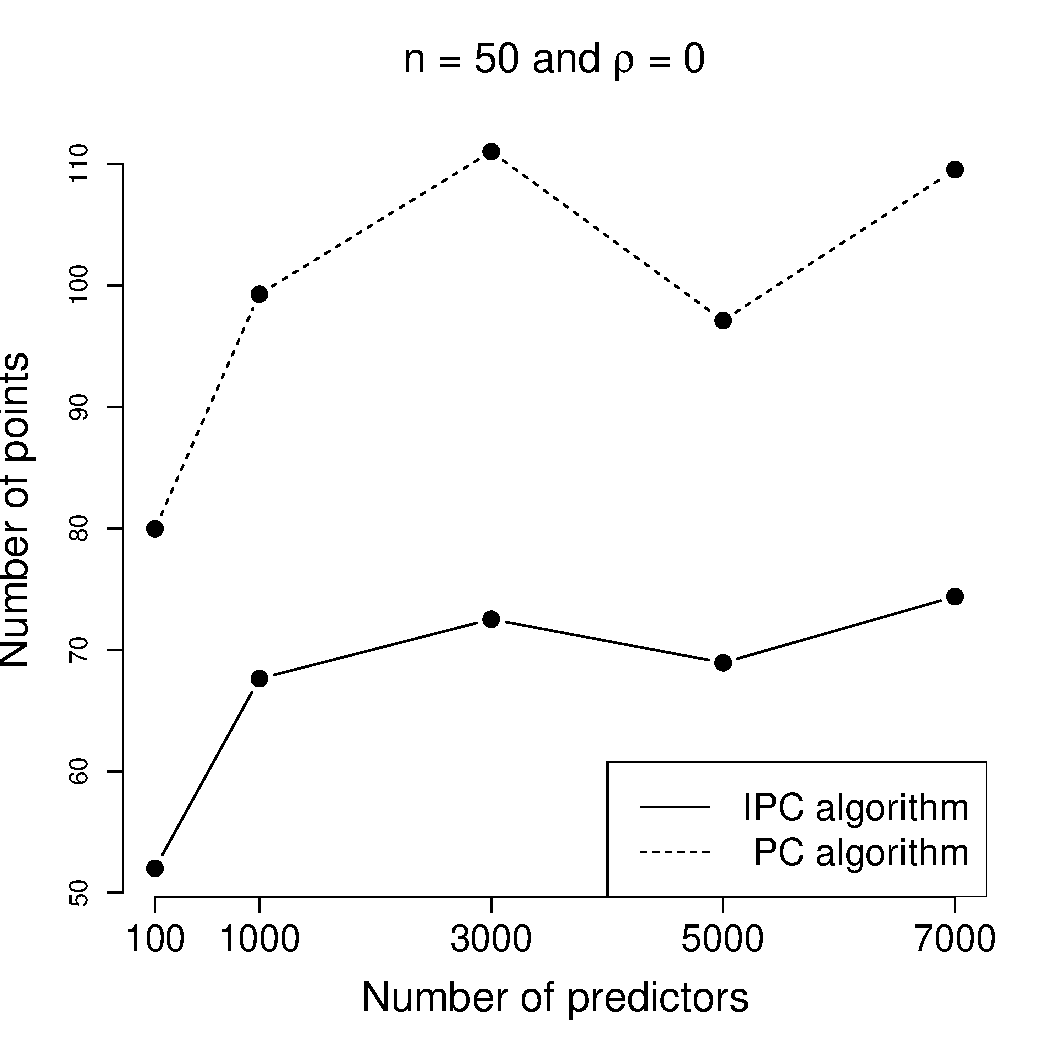
\includegraphics[width=0.47\textwidth]{n50_rho0.pdf}}
	{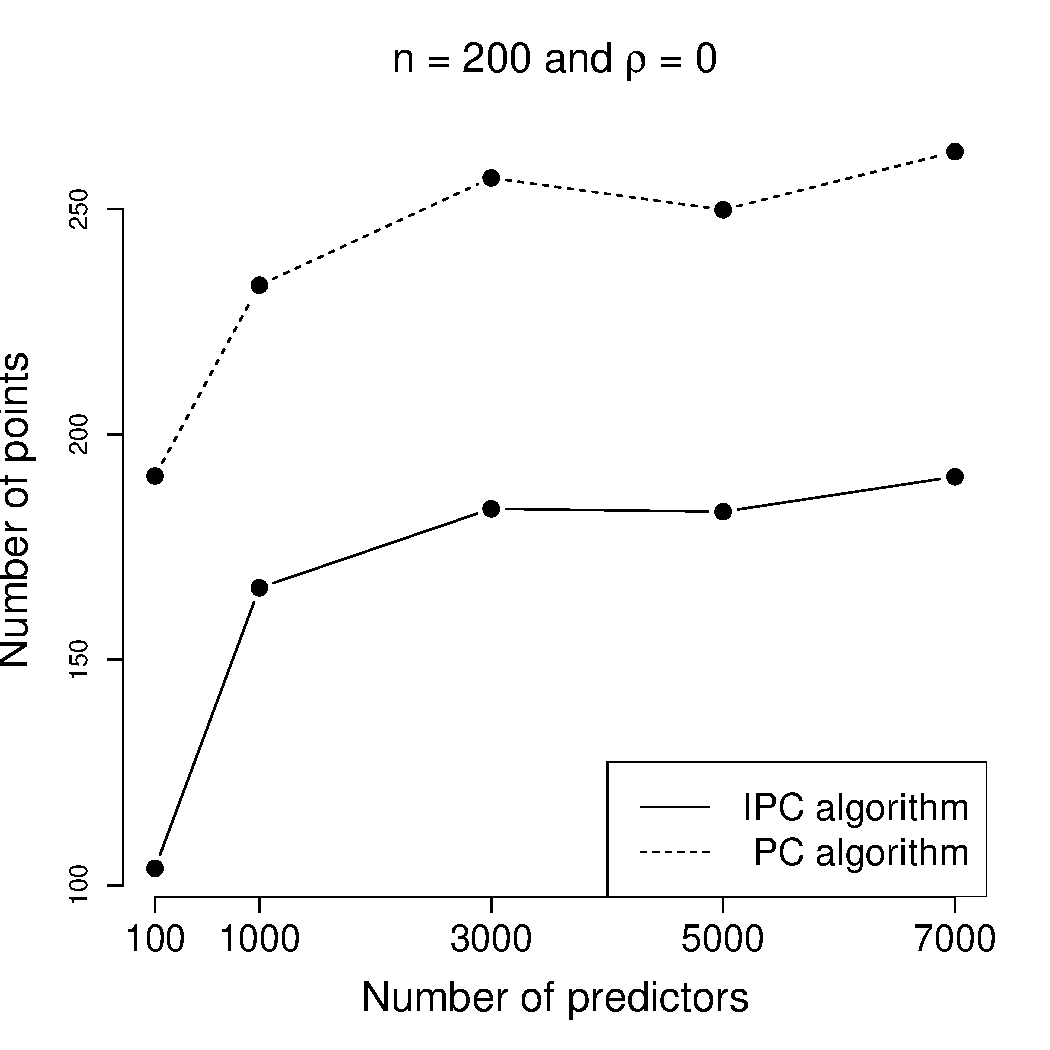
\includegraphics[width=0.47\textwidth]{n200_rho0.pdf}}
	{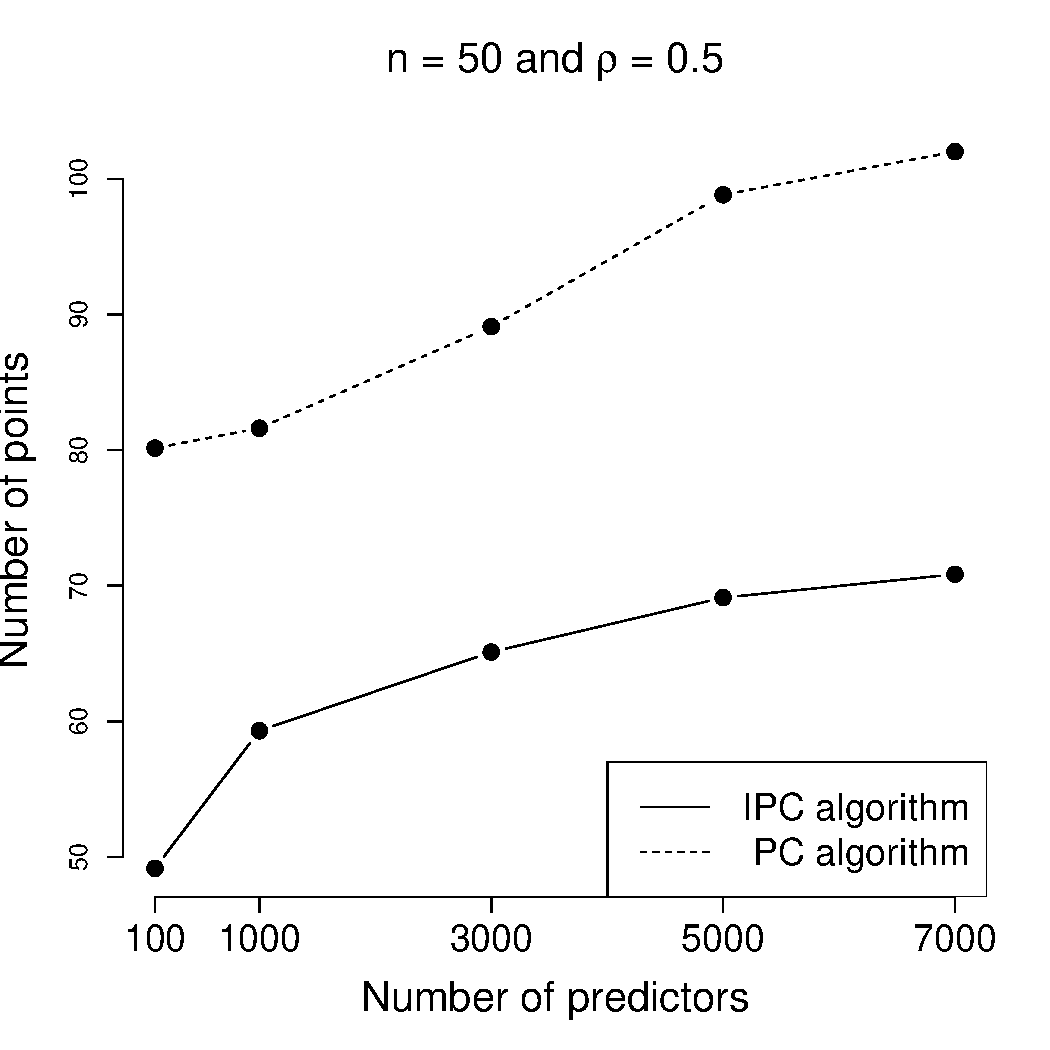
\includegraphics[width=0.47\textwidth]{n50_rho05.pdf}}
	{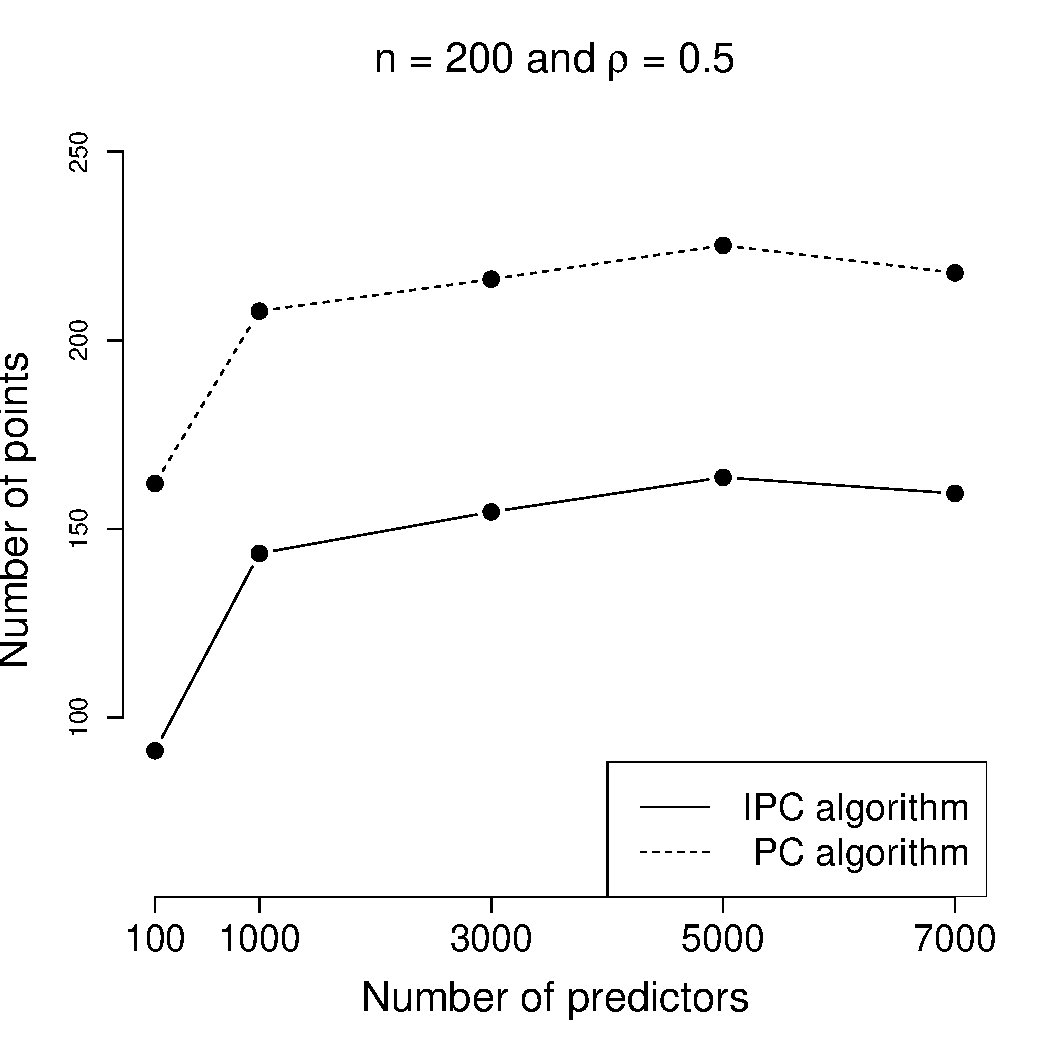
\includegraphics[width=0.47\textwidth]{n200_rho05.pdf}}
	\caption{Simulation study for a logistic regression showing the relationship between the trimmed mean number of points of the solution curve $q$ for the IPC and PC algorithms at the 5\% level. In all cases, the IPC algorithm is faster than the PC.}
	\label{fig:cpu}
\end{figure}



Our simulation study is based on a logistic regression model with sample size equal to $n=50, 200$. The number of predictors $p$ follows a sequence of five values 100, 1000, 3000, 5000 and 7000. The study is based on two different configurations of the covariance structure of the $ p $ predictors, that is, the random vector $X=(X_1, X_2, \cdots ,X_p)^\top$ is sampled from an $ N (\boldsymbol{0}, \Sigma) $ distribution with elements of $ \Sigma $ satisfying $corr(X_i;X_j)=\rho^{|i-j|}$, where $\rho=0$ or $\rho= 0.5$. The response vector is simulated using a model with intercept $\beta_0$ and regression coefficients $\bm\beta$ chosen as follows:
%
\begin{align*}
\beta_0 = 1\quad\text{and}\quad\boldsymbol{\beta}=(1, 2, 3, \underset{p-3}{\underbrace{0, \cdots, 0}}).
\end{align*}
%
The \code{R} code to replicate our study is reported in the attached file. Table \ref{tab:cpu} reports the average CPU times in seconds and the mean number of points of the solution curve ($q$) coming from $100$ simulation runs, so that all means and their standard deviations are trimmed of the 5\% tails. All timings reported were carried out on a personal computer with Intel Core $i5 \ 520M$ dual-core processor. 
%Since both the IPC and PC algorithms have been written in {Fortran 90}, it can be seen that they are  almost equal in terms of CPU time. 
%When we deal with high-dimensional data (e.g. $p=7000$ and $n=200$), 
The proposed IPC algorithm is always faster than the PC algorithm, regardless of the correlation between the predictors. This table also displays that, the trimmed mean number of the points of the solution curve yielded by the IPC algorithm is always lower than those needed in the PC algorithm. 
%Thus, we clearly see that the proposed IPC algorithm is always faster than the PC algorithm. The differences between the two algorithms are tangible when $\rho=0$ (no correlation among the predictors). 
Interestingly, when the correlation among the predictors is stronger ($\rho=0.5$) both algorithms are faster than when there is no correlation. Figure~\ref{fig:cpu} shows the trimmed mean number of the points of the solution curve for the two algorithms. The IPC algorithm is more efficient than the PC algorithm. 


\section[Application to Example Data]{Application to Example Data}
\label{sec:realdata}


In this section we analyze an example dataset by using the functions available in the \CRANpkg{dglars} package. We consider the benchmark \texttt{diabetes} data  \citep{efron04} to study the sparse structure of an inverse Gaussian regression model. This dataset was also used in \cite{ish10a} and is  available in the {R} package \CRANpkg{lars}:
%
\begin{example}
R> install.packages(pkgs = "lars")
R> data("diabetes", package = "lars")
\end{example}
%
The response $y$ are quantitative measurements of disease progression for patients with diabetes after one year. The covariate data include 10 baseline measurements for each patient, recorded in the design matrix \code{x}, such as \textit{age}, \textit{sex}, \textit{bmi} (body mass index), \textit{map} (mean arterial blood pressure) and six blood serum measurements: \textit{ldl} (low-density lipoprotein), \textit{hdl} (high-density lipoprotein), \textit{ltg} (lamotrigine), \textit{glu} (glucose), \textit{tc} (triglyceride) and \textit{tch} (total cholesterol). In addition to $\binom{10}{2} = 45$ interactions and 9 quadratic terms (excluding the binary sex variable), the design matrix \code{x2} consists of a total of 64 columns. So, the complete data consists of  diabetes progression observations on $n=442$ patients in combination with $p=64$ predictor variables.  The aim of the study is to identify which of the covariates are important factors in disease progression. 


From previous analyses, it was clear that the disease progression is not appropriately modelled by a Gaussian. After some goodness-of-fit considerations, we settle on an inverse Gaussian regression model, which requires us to estimate the dispersion parameter. First, we estimate the optimal value of the tuning parameter $\gamma$ by 10-fold cross-validation (CV) using the \code{cvdglars()} function, i.e.,

\begin{example}
R> library("dglars")
R> set.seed(11235)
R> cv_diabetes <- cvdglars(y ~ x, family = inverse.gaussian("log"), 
+                          data = diabetes)
R> cv_diabetes

Call:  cvdglars(formula = y ~ x, family = inverse.gaussian("log"), data = diabetes)

Coefficients:
     Estimate
Int.   4.9539
xsex  -2.0273
xbmi   2.8447
xmap   2.1969
xtc   -0.3811
xhdl  -2.4124
xltg   3.8501

Dispersion parameter: 0.001141

Details:
   number of non zero estimates: 8
      cross-validation deviance: 0.06224
                              g: 0.01533
                        n. fold: 10

Algorithm 'pc' ( method = 'dgLASSO' )
\end{example}

This output shows that the dgLARS method by the help of the CV criterion selects an inverse Gaussian regression model with six covariates (\textit{sex}, \textit{bmi}, \textit{map}, \textit{tc}, \textit{hdl} and \textit{ltg});

\begin{example}
R> cv_diabetes$formula_cv
y ~ sex + bmi + map + tc + hdl + ltg
\end{example}
%five predictors (\textit{sex}, \textit{bmi}, \textit{map}, \textit{hdl} and \textit{ltg})
Moreover, the optimal tuning parameter is $\gamma=0.01533$ and the dispersion parameter estimate by the GRCV method is $\hat{\phi}_{GRCV}=0.001141$. If we had selected the BIC instead of 10-fold cross-validation, we would have obtained

\begin{example}
R> diabetes_dglars <- dglars(y ~ x, family = inverse.gaussian("log"),
+                            data = diabetes)
R> set.seed(11235)
R> summary(diabetes_dglars, type = "BIC", phi = "grcv")

Call:  dglars(formula = y ~ x, family = inverse.gaussian("log"), data = diabetes)

  Sequence         g     %Dev  df   BIC   Rank
            0.505974  0.00000   2  5223  18   
   + xbmi                                     
            0.481473  0.02290   3  5207  17   
            0.481262  0.02309   3  5207  16   
   + xltg                                     
            0.250152  0.26744   4  4986  15   
            0.233248  0.27846   4  4975  14   
            0.233174  0.27851   4  4975  13   
   + xmap                                     
            0.222313  0.28613   5  4974  12   
   + xhdl                                     
            0.100212  0.36560   6  4906  11   
            0.099904  0.36572   6  4906  10   
   + xsex                                     
            0.030320  0.41322   7  4868   2   
            0.030263  0.41324   7  4868   1 <-
    + xtc                                     
            0.014883  0.41892   8  4869   3   
   + xglu                                     
            0.005757  0.42063   9  4873   4   
   + xtch                                     
            0.002389  0.42122  10  4879   6   
            0.002384  0.42122  10  4879   5   
   + xldl                                     
            0.001704  0.42199  11  4884   8   
            0.001691  0.42200  11  4884   7   
   + xage                                     
            0.000001  0.42272  12  4890   9   

Details:
	 BIC values computed using k = 6.091 and complexity = 'df'
	 dispersion parameter estimated by 'grcv'

===============================================================

Summary of the Selected Model

    Formula: y ~ xsex + xbmi + xmap + xhdl + xltg
     Family: 'inverse.gaussian'
       Link: 'log'

Coefficients:
     Estimate
Int.   4.9495
xsex  -1.6834
xbmi   2.7786
xmap   1.9536
xhdl  -2.2917
xltg   3.5420

Dispersion parameter: 0.001112 (estimated by 'grcv' method)
---

                 g: 0.03026
     Null deviance:    1.0361 
 Residual deviance:    0.6079 
               BIC: 4868.0435 

 Algorithm 'pc' ( method = 'dgLASSO' )
\end{example}

The fitted model now does not include \emph{tc}, but does include the other five predictors (\textit{sex}, \textit{bmi}, \textit{map}, \textit{hdl} and \textit{ltg}). In fact, the optimal value of the tuning parameter $\gamma=0.03026$ is somewhat larger than with cross-validation, as can be expected from the BIC, resulting in a sparser model. The GRCV estimate of the dispersion parameter $\hat{\phi}_{GRCV}= 001112$, due to the stable nature of the GRCV method. It is also possible to obtain the GRCV estimate directly without a fitted `\code{dglrs}' object, by only using the design matrix \code{x} and the response variable \code{y} using the following  code:

\begin{example}
set.seed(11235)
grcv(diabetes_dglars, type = "BIC")

[1] 0.001111604
\end{example}

Since the original PC algorithm is only available for the version $1.0.5$ (and older) and the inverse Gaussian family has only been  added to the package from  version $2.0.0$ onwards, we are not able to compare the run times and also the number of the iterations computing the solution points for the PC and IPC algorithms. The run time of the IPC algorithm is given using the following {R} code:

\begin{example}
R> system.time(diabetes_dglars_ipc <- dglars(y ~ x, 
+              family = inverse.gaussian("log"), data = diabetes))

user  system elapsed 
0.016   0.000   0.016 
\end{example}
and the number of iterations computing the solution points by the IPC algorithm is
\begin{example}
R> diabetes_dglars_ipc$np

[1] 18
\end{example}

\section[Conclusions]{Conclusions}
\label{sec:conclu}


In this paper, we have described improvements to the {R} package \CRANpkg{dglars} for estimating a larger class of generalized linear models with arbitrary link functions and a general class of exponential dispersion models. 
We briefly reviewed the differential geometrical theory underlying the dgLARS method and briefly explained the dispersion parameter estimation methods. We described some functions implemented in the new version of the \CRANpkg{dglars} package that can be used to estimate the dispersion parameter. We also used these functions to compare run times between the new IPC and old PC algorithms. 
The simulations showed that the IPC algorithm is significantly faster than the original PC algorithm. The new version of \CRANpkg{dglars} is available on CRAN.

\section*{Acknowledgments}
This article is based upon work from COST Action \emph{European Cooperation for Statistics of Network Data Science} (COSTNET, CA15109), supported by COST
(European Cooperation in Science and Technology).









\bibliography{pazira}


\address{Hassan Pazira\\
	Epidemiology and Biostatistics\\
	VU University Medical Center\\
	De Boelelaan 1117, 1081 HV Amsterdam, The Netherlands\\
	\email{h.pazira@amsterdamumc.nl}}

\address{Luigi Augugliaro\\
	Department of Economics, Business and Statistics\\
	University of Palermo\\
	90128 Palermo, Italy\\
	\email{luigi.augugliaro@unipa.it}}

\address{Ernst C. Wit \\
	Institute of Computational Science\\
	Universit\`a della Svizzera italiana (USI)\\
	Via G. Buffi 13, 6900 Lugano, Switzerland\\
	\email{wite@use.ch}}

\end{article}

\end{document}
